\documentclass{beamer}
\usepackage{graphicx}
\usepackage{hyperref}
\usepackage{mathtools}
\usepackage{tikz}

\title{Collective motion of squirmers in confined
environments}
\author{Robin Roth}
\institute{Supervised by: Van Landeghem Céline, Giraldi Laetitia, Agathe Chouippe}
\date{August 23, 2024}

\begin{document}
\begin{frame}
    \titlepage
\end{frame}

\begin{frame}{Table of contents}
    \tableofcontents
\end{frame}

\section{What is a squirmer ?}
\begin{frame}{What is a squirmer ?}
    \begin{columns}[T]
        \begin{column}{0.5\textwidth}
            \begin{itemize}
                \item Introduced by James Lighthill in 1952 \cite{Wikipedia}
                \item Extended by John Blake in 1971 \cite{Wikipedia}
                \item Model for a spherical microswimmer
                \item Cannot model cilia so we impose boundary conditions
                \begin{itemize}
                    \item Tangential time-independant velocity at the boundary, propelling the squirmers.
                    \item In particullar, we fix the type $\beta$ and the velocity $B_1$.
                \end{itemize}
            \end{itemize}
        \end{column}
        \begin{column}{0.5\textwidth}
            \centering
            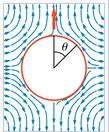
\includegraphics[width=\textwidth]{../images/squirmer.png}
            \cite{Wikipedia}
        \end{column}
    \end{columns}
\end{frame}

\section{Objectives}
\begin{frame}{Objectives}
    \begin{itemize}
        \item Update the torques' and forces' formulas.
        \item Investigate the impact of the $\beta$ parameter on the interaction
        \begin{itemize}
            \item between two squirmers.
            \item between a squirmer and a wall.
        \end{itemize}
        \item Update and vectorize the code to simulate a large number of squirmers.
        \item Examine the impact of numerical parameters on the collective behavior of squirmers.
    \end{itemize}
\end{frame}

\section{Roadmap}
\begin{frame}{Roadmap}
    \begin{center}
        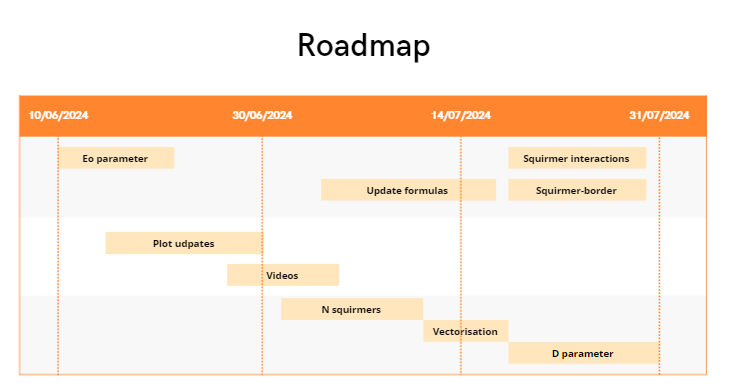
\includegraphics[width=0.9\textwidth]{../images/roadmap_stage.png}
    \end{center}
\end{frame}

\section{Squirmer model}
\begin{frame}{Squirmer model}
    \begin{center}
        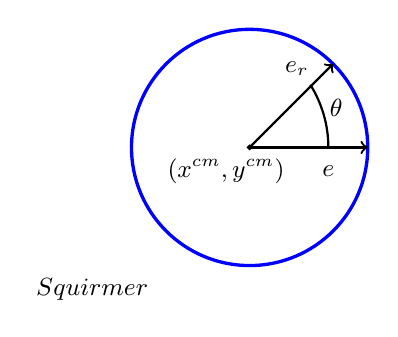
\begin{tikzpicture}
        \small
        
        \draw[color=blue, very thick](2.5,2.5) circle (1.5);
        
        \draw[color=black, very thick](2.5,2.5) circle (0.01);
        
        \node  at (2.5-0.3,2.5-0.3) {{$(x^{cm},y^{cm})$}};
        
        \node  at (0.5,0.7) {{$Squirmer$}};
        
        \draw[thick, ->] (2.5,2.5) -- (4,2.5);
        \node  at (3.5,2.2) {{$e$}};
     
        \pgfmathsetmacro{\xcoord}{2.5 + 1.5*cos(45)}
         \pgfmathsetmacro{\ycoord}{2.5 + 1.5*sin(45)}
         \draw[thick, ->] (2.5,2.5) -- (\xcoord,\ycoord);
        \node  at (3.1,3.5) {{$e_r$}}; 
        \draw[thick, -] (3.5,2.5) arc[start angle=0, end angle=32, radius=1.5];
        \node at (3.6,3) {${\theta}$}; 
        
           
        \end{tikzpicture}
        \end{center}
    \begin{itemize}
        \item The velocity $u$ in polar coordinates \cite{Lauga} : \begin{align*}
       \left\{\begin{array}{rcl}
          u_r(R,\theta) &=& 0 \\
          u_\theta(R,\theta) &=& B_1(\mathrm{sin}(\theta) + \beta \mathrm{sin}(\theta)\mathrm{cos}(\theta)), B_1 = \frac{3}{2}v_0
       \end{array}\right.\;
        \end{align*} with $\beta=\frac{B_2}{B_1}$ :
    $\left\{
        \begin{array}{ll}
            \beta = 0 : \text{neutral swimmer}  \\
            \beta < 0 : \mathrm{pusher} \\
            \beta > 0 : \mathrm{puller} \\
        \end{array}
    \right.$
        \item In  cartesian coordinates :
        $u_r = B_1(1+\beta (e\cdot e_r)) [(e\cdot e_r)e_r - e]$
    \end{itemize}
\end{frame}
    
\section{Dynamics of two interacting squirmers}
\subsection{The evolution of the mass center $r_i$}    
\begin{frame}{Dynamics of two interacting squirmers}
        \framesubtitle{The evolution of the mass center $r_i$}
        The evolution of the mass center $r_i$ = $(X_i, Y_i)$ of one squirmer $i$ in presence of 
    another squirmer $j$ and rigid boundaries, is given by :
    \begin{center}
        \footnotesize
        $\boxed{\frac{dr_i}{dt}$ = $v_0 p_i -  \sum\limits_{i \ne j}\nabla_{r_{ij}} V_{ij} - \sum\limits_{i}\nabla_{r_i} V_i + \sum\limits_{i\ne j}\left[F_{i(j)\rightarrow i} + F_{j(i)\rightarrow i}\right]+ \sum\limits_{k \in w}F_{k\rightarrow i}^w + \sqrt{2D}\eta_i(t)}$
    \end{center}
    \normalsize
    We have : \begin{itemize}
        \item $v_0$ the particle velocity,
    \item $p_i$ = $(\mathrm{cos}(\theta),\mathrm{sin}(\theta))^T$ orientation,
    \item $F_{i(j)\rightarrow k}$, the lubrification forces applied on the $k^{th}$ squirmer and generated by the $i^{th}$ squirmer in presence of the $j^{th}$ one \cite{Brumley},
    \item $F^w_{k\rightarrow i}$, the lubrification forces exerted on the $i^{th}$ squirmer due to the presence of the $k^{th}$ wall\cite{Brumley},
    \item $V_{ij}$ and $V_i$ the Weeks-Chandler-Andersen potential,
    \item $D$ the translational diffusivity,
    \item $\eta_i$ are independent noises. 
    \end{itemize}
\end{frame}

\begin{frame}
    \framesubtitle{The evolution of the mass center $r_i$}
    The second law of Newton\cite{Newton}:
    $$m\vec{a} = \sum\limits_i \vec{F}_i.$$
    The force of viscosity on a small sphere moving through a viscous fluid is given by the Stokes-Einstein relation\cite{Stokes}:
    $$F_d = 6\mu\pi Rv_0\frac{dr_i}{dt}.$$
    We consider the squirmers propulsion in absence of inertia: $m\vec{a} = 0$. One has:
    $$0 = -F_d + \sum\limits_{i \ne d} F_i,$$
    we have:
    $$\frac{dr_i}{dt} = \frac{1}{6\mu\pi R}\sum\limits_{i \ne d} F_i.$$
\end{frame}
    
\begin{frame}{Dynamics of two interacting squirmers}
    \framesubtitle{The evolution of the mass center $r_i$}
    \begin{center}
        \footnotesize
        $\boxed{\frac{dr_i}{dt} = v_0 p_i -  \sum\limits_{i \ne j}\nabla_{r_{ij}} V_{ij} - \sum\limits_{i}\nabla_{r_i} V_i + \sum\limits_{i\ne j}\left[F_{i(j)\rightarrow i} + F_{j(i)\rightarrow i}\right]+ \sum\limits_{k \in w}F_{k\rightarrow i}^w + \sqrt{2D}\eta_i(t)}$
    \end{center}
    We have: 
    \begin{itemize}
        \item $\nabla_{r_{ij}} V_{ij}$ = 
        $\begin{pmatrix}
            -\frac{E_s}{2R^2\pi\mu} \frac{D_x}{r_{ij}}\left[ \frac{2(2R)^{13}}{(r_{ij})^{13}} - \frac{(2R)^7}{(r_{ij})^7} \right] \\
            -\frac{E_s}{2R^2\pi\mu} \frac{D_y}{r_{ij}}\left[ \frac{2(2R)^{13}}{(r_{ij})^{13}} - \frac{(2R)^7}{(r_{ij})^7} \right]
        \end{pmatrix}$
        \item $\nabla_{r_i} V_i$ = $\begin{pmatrix}
            - \frac{E_s (X_{box}-X)}{\pi\mu R^2 \lvert r - r_i \rvert } \left[ 2 \left( \frac{R}{\lvert r-r_i\rvert} \right)^{13} - \left( \frac{R}{\lvert r-r_i\rvert}\right)^7 \right] \\
            - \frac{E_s (Y_{box}-Y)}{\pi\mu R^2 \lvert r - r_i \rvert } \left[ 2 \left( \frac{R}{\lvert r-r_i\rvert} \right)^{13} - \left( \frac{R}{\lvert r-r_i\rvert}\right)^7 \right]
        \end{pmatrix}$
    \end{itemize}
\end{frame}


\begin{frame}{Dynamics of two interacting squirmers}
    \begin{center}
        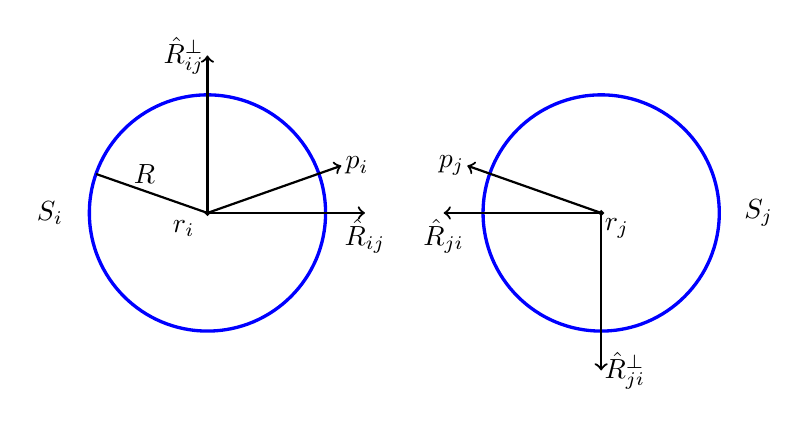
\begin{tikzpicture}

            \draw[color=blue, very thick](5,5) circle (1.5);
            \draw[color=blue, very thick](0,5) circle (1.5);
            
            \draw[color=black, very thick](0,5) circle (0.01);
            \draw[color=black, very thick](5,5) circle (0.01);
            
            \node  at (-0.3,5-0.2) {{$r_i$}};
            \node  at (5+0.2,5-0.2) {{$r_j$}};
            
            \node  at (-2,5) {{$S_i$}};
            \node  at (7,5) {{$S_j$}};
            
            \draw[thick, ->] (0,5) -- (1.7,5+0.6);
            \draw[thick, ->] (5,5) -- (5-1.7,5+0.6);
            
            \node  at (1.9,5+0.6) {{$p_i$}};
            \node  at (5-1.9,5+0.6) {{$p_j$}};
            
            \draw[thick] (0,5) -- ({-cos(45)*2}, {5+0.7*sin(45)});
            \node  at (-0.8,5+0.5) {{$R$}};
            
            \draw[thick, ->] (0,5) -- (2,5);
            \draw[thick, ->] (5,5) -- (3,5);
            
            \node  at (2,5-0.3) {{$\hat{R}_{ij}$}};
            \node  at (3,5-0.3) {{$\hat{R}_{ji}$}};
            
            \draw[thick, ->] (0,5) -- (0,7);
            \node  at (-0.3,7) {$\hat{R}_{ij}^{\perp}$};
            
            
            \draw[thick, ->] (5,5) -- (5,3);
            \node  at (5.3,3) {$\hat{R}_{ji}^{\perp}$};
            
            \end{tikzpicture}
    \end{center}
    The figure shows the different vectors involved in the computations which will follow.
        
\end{frame}
    
\begin{frame}{Dynamics of two interacting squirmers}
    \begin{itemize}
        \item The tangential lubrification forces acting on the two spheres : \begin{equation*}
            \boxed{
F_{i(j)\rightarrow i}^{y} = -\frac{9}{16}v_0
\left[(p_i\hat{R}_{ij})(1 + \beta p_i\hat{R}_{ij}) - \frac{1}{2}\beta(p_i\hat{R}^{\perp}_{ij})^2\right](ln \epsilon + O(1))
}
\end{equation*}
    \item The normal forces acting on the two spheres :
    \begin{equation*}
\boxed{F_{i(j)\rightarrow i}^{x} = -\frac{1}{4}v_0p_i\hat{R}^{\perp}_{ij}(1 + \beta p_i\hat{R}_{ij})(ln \epsilon + O(1))}
\end{equation*}
    \item The effect of a wall can be calculated by replacing one of the spheres with one of infinite diameter, so $\lambda\rightarrow\infty$:
    \begin{equation*}
        \boxed{F_{w\rightarrow i}^{y} = -\frac{9}{4} v_0
        \left[(p_i\hat{R}_{ij})(1 + \beta p_i\hat{R}_{ij}) - \frac{1}{2}\beta(p_i\hat{R}^{\perp}_{ij})^2\right](ln \epsilon + O(1))}
    \end{equation*}
    \begin{equation*}
        \boxed{F_{w\rightarrow i}^{x} = -\frac{1}{5} v_0p_i\hat{R}^{\perp}_{ij}(1 + \beta p_i\hat{R}_{ij})(ln \epsilon + O(1))}
    \end{equation*}
    \end{itemize}
\end{frame}
    
\subsection{The evolution of the orientation $\theta _i$}
\begin{frame}{Dynamics of two interacting squirmers}
        \framesubtitle{The evolution of the orientation $\theta _i$}
    The evolution of the rotation of one squirmer is given by : 
    $$
    \frac{d \theta_i}{dt} = \sum\limits_{i\ne j} \left[\Gamma_{i(j)\rightarrow i} + \Gamma_{j(i)\rightarrow i}\right] + \sum\limits_{k\in w} \Gamma_{k\rightarrow i}^w + \sqrt{2D_o} \eta_o^{(i)}.
    $$ 
    \begin{itemize}
        \item $\Gamma_{i(j)\rightarrow k}$ the torque exerted on the $k^{th}$ particle by the flow associated to the $i^{th}$ particle, but perturbed by the presence of the $j^{th}$ particle,
        \item $\Gamma_{k\rightarrow i}^w$ the torque exerted on the $i^{th}$ particle by the interactions with the $k^{th}$ walls,
        \item $D_o$ the angular diffusivity equal to $\frac{3D}{4R^2}$,
        \item $\eta_o^{(i)}$ the noises, independent of $\eta^{i}$.
    \end{itemize}
\end{frame}

\begin{frame}
    $\phi = 8\pi\mu r^3$ the rotation flow around a sphere\cite{Stokes}:
$$\frac{d \theta_i}{dt} = \frac{1}{\phi}\sum F\cite{Newton}.$$
    \begin{itemize}
        \item The torques acting on the squirmer $i$ :
        \begin{equation*}
        \boxed{\Gamma_{i(j)\rightarrow i} = \frac{3}{10}\frac{v_0}{R}p_i\hat{R}_{ij}^{\perp}(1 + \beta p_i\hat{R}_{ij})(ln \epsilon + O(1))}
    \end{equation*}
        \item The torques acting on the squirmer $j$ :
        \begin{equation*}
        \boxed{\Gamma_{i(j)\rightarrow j} = \frac{3}{40}\frac{v_0}{R}p_i\hat{R}_{ij}^{\perp}(1 + \beta p_i\hat{R}_{ij})(ln \epsilon + O(1))}
    \end{equation*}
        \item The torques produced by the walls on the squirmer $i$:
        \begin{equation*}
            \boxed{\Gamma_{w\rightarrow i} = \frac{3}{5} \frac{v_0}{R}p_i\hat{R}_{ij}^{\perp}(1 + \beta p_i\hat{R}_{ij})(ln \epsilon + O(1))}
        \end{equation*}
    \end{itemize}
        
\end{frame}

\section{Implementation in Python}
\begin{frame}{Implementation in Python}
\begin{center}
    \footnotesize
        \(\boxed{\frac{dr_i}{dt} = v_0 p_i -  \sum\limits_{i \ne j}\nabla_{r_{ij}} V_{ij} - \sum\limits_{i}\nabla_{r_i} V_i + \sum\limits_{i\ne j}\left[F_{i(j)\rightarrow i} + F_{j(i)\rightarrow i}\right]+ \sum\limits_{k \in w}F_{k\rightarrow i}^w + \sqrt{2D}\eta_i(t)}\)
\end{center}
\begin{center}
    \footnotesize
        \(\boxed{\frac{d \theta_i}{dt} = \sum\limits_{i\ne j} \left[\Gamma_{i(j)\rightarrow i} + \Gamma_{j(i)\rightarrow i}\right] + \sum\limits_{k\in w} \Gamma_{k\rightarrow i}^w + \sqrt{2D_o} \eta_o^{(i)}}\)
\end{center}
\normalsize
\begin{itemize}
    \item Steric forces:
    \begin{itemize}
        \item if $\lvert r_i-r_j\rvert < 2^{\frac{7}{6}}R$, we add $\nabla_{r_{ij}}V_{ij}$
        \item if $\lvert B-r_i\rvert < 2^{\frac{1}{6}}R$, we add $\nabla_{r_{i}}V_{i}$
    \end{itemize}
    \item Lubrification forces:
    \begin{itemize}
        \item if $\lvert r_i-r_j\rvert < 3R$, we add $F_{i(j)\rightarrow i}$ and $\Gamma_{i(j)\rightarrow i}$ to the $i^{th}$ squirmer, and $F_{i(j)\rightarrow j}$ and $\Gamma_{i(j)\rightarrow j}$ to the $j^{th}$
        \item if $\lvert B-r_i\rvert < 2R$, we add $F_{k\rightarrow i}^w$ and $\Gamma_{k\rightarrow i}^w$
    \end{itemize}
\end{itemize}
\end{frame}

\section{Numerical Experiments}
\begin{frame}{Numerical Experiments}
    \begin{center}
        Results from previous study \cite{Stark}
        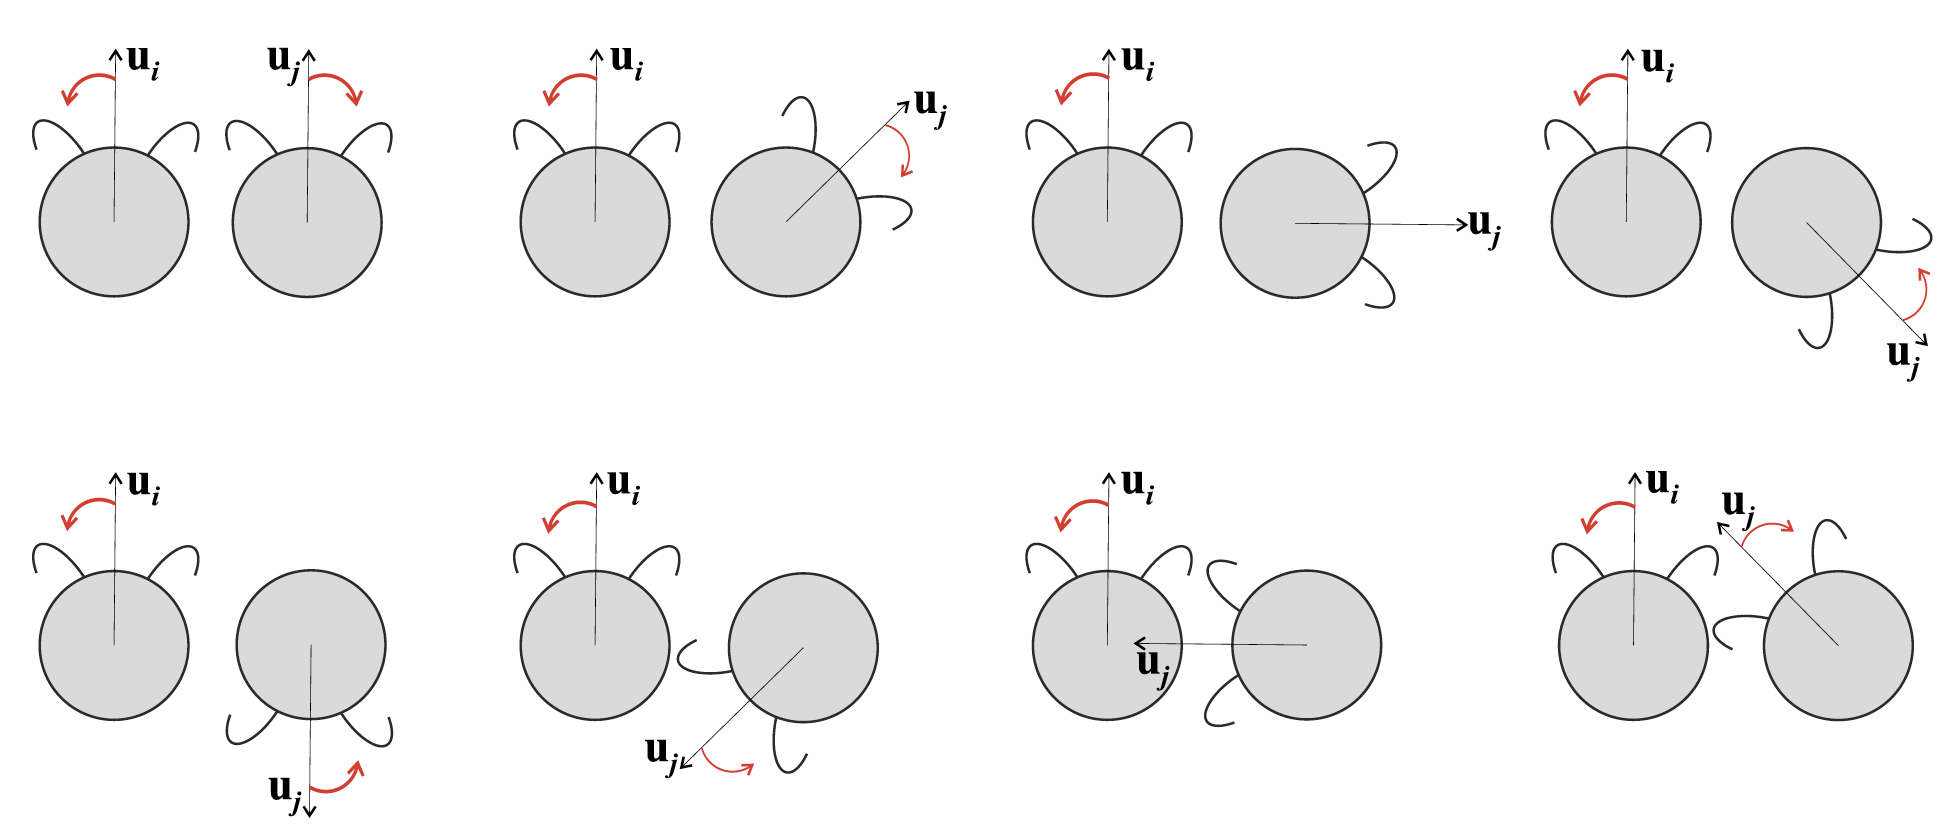
\includegraphics[width=0.8\textwidth]{../images/stark_behavior.png}
        \cite{Stark}
    \end{center}
\end{frame}

\subsection{Simulation of two interacting squirmers}
\begin{frame}{Numerical Experiments}
    \framesubtitle{Simulation of two interacting squirmers}
    \begin{center}
        \textbf{$\theta_2 = \frac{3\pi}{4}$}
    \end{center}
    \begin{minipage}{0.49\textwidth}
        \centering
        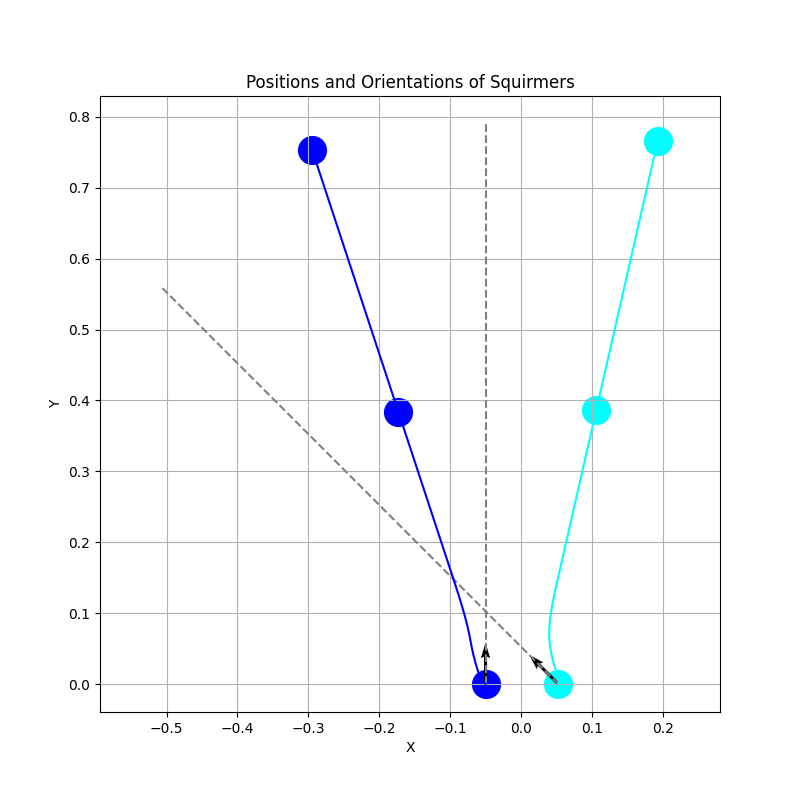
\includegraphics[width=1\textwidth]{../../graphs/simulations/sim_sq_sq/betam1_5/3pi_4_.png}
        $\beta = -1.5$
    \end{minipage}
    \begin{minipage}{0.49\textwidth}
        \centering
        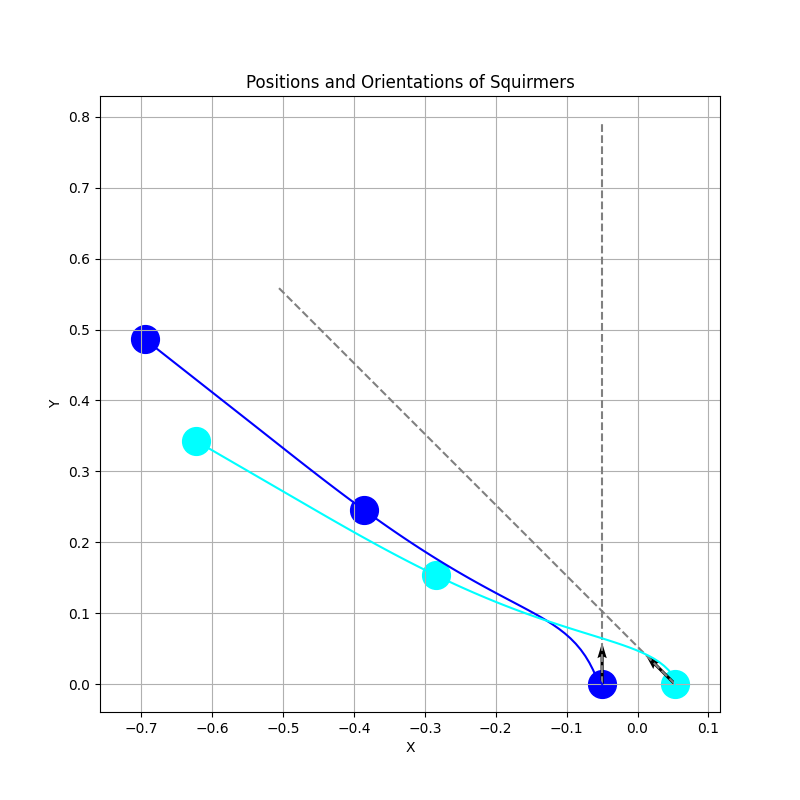
\includegraphics[width=1\textwidth]{../../graphs/simulations/sim_sq_sq/beta1_5/3pi_4_.png}
        $\beta = 1.5$
    \end{minipage}
\end{frame}

\begin{frame}{Numerical Experiments}
    \framesubtitle{Simulation of two interacting squirmers}
    \centering
    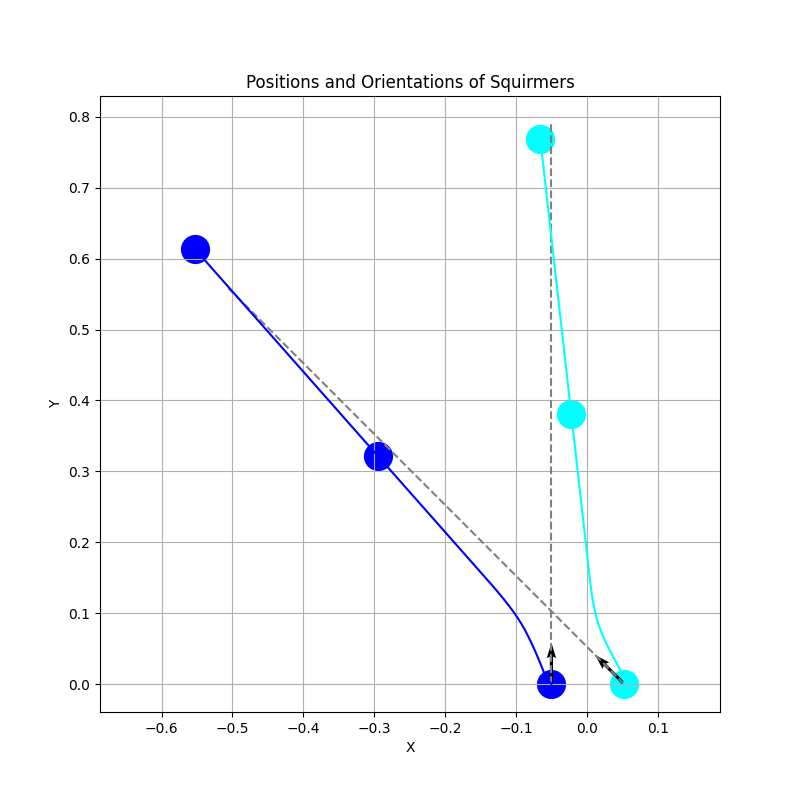
\includegraphics[width=0.5\textwidth]{../../graphs/simulations/sim_sq_sq/beta0/3pi_4_.png}
    \begin{center}
        $\beta = 0$
    \end{center}
\end{frame}

\begin{frame}{Numerical Experiments}
    \framesubtitle{Simulation of two interacting squirmers}
    \begin{center}
        Two different positive $\beta$ values
    \end{center}
    \begin{minipage}{0.49\textwidth}
        \centering
        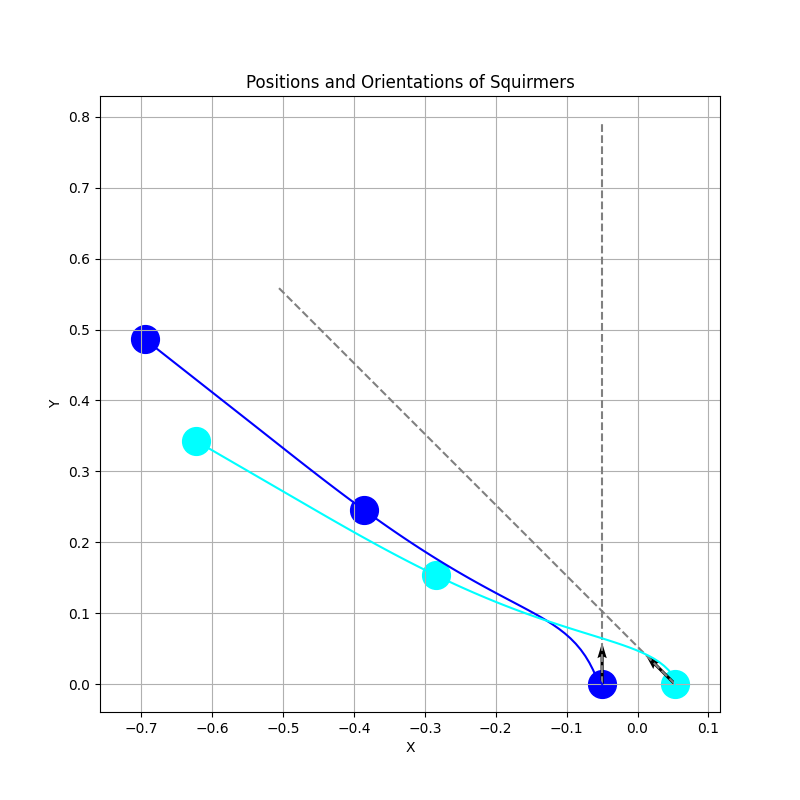
\includegraphics[width=1\textwidth]{../../graphs/simulations/sim_sq_sq/beta1_5/3pi_4_.png}
        $\beta = 1.5$
    \end{minipage}
    \begin{minipage}{0.49\textwidth}
        \centering
        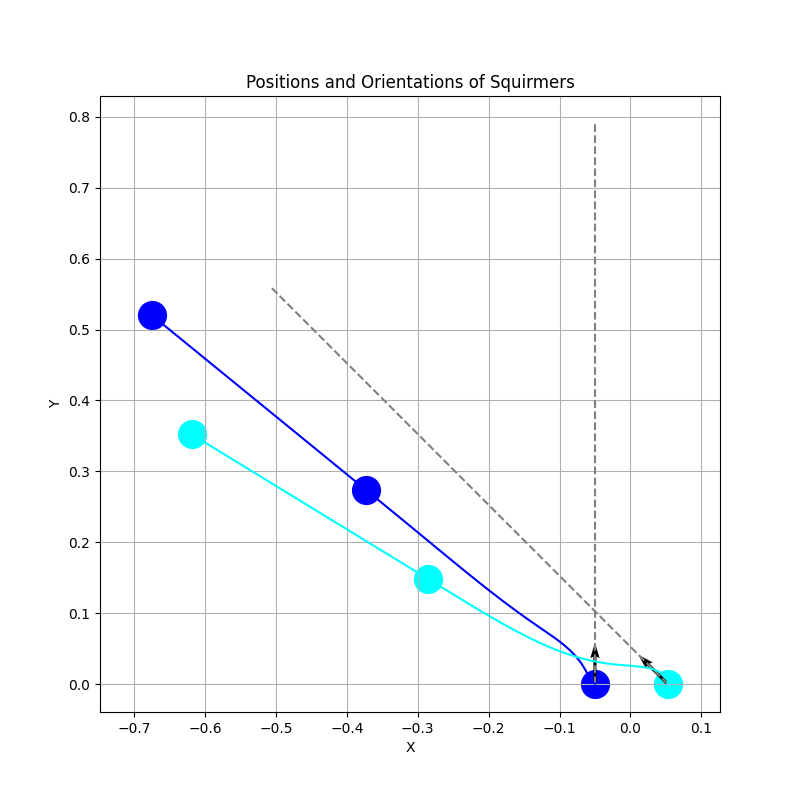
\includegraphics[width=1\textwidth]{../../graphs/simulations/sim_sq_sq/beta3/3pi_4_.png}
        $\beta = 3$
    \end{minipage}
\end{frame}

\begin{frame}{Numerical Experiments}
    \framesubtitle{Simulation of two interacting squirmers}
    \begin{center}
        Two different negative $\beta$ values
    \end{center}
    \begin{minipage}{0.49\textwidth}
        \centering
        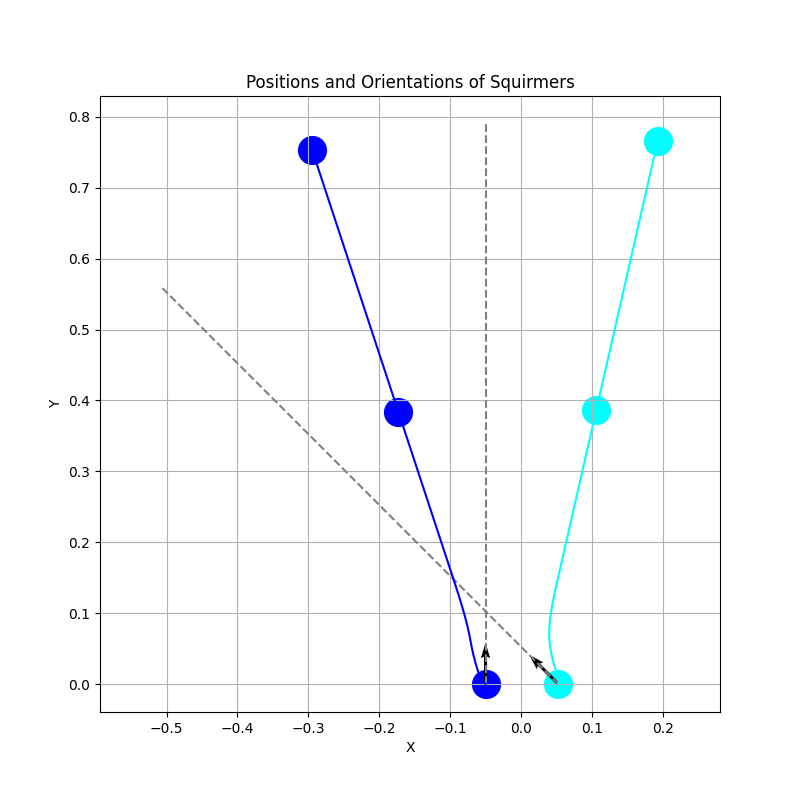
\includegraphics[width=1\textwidth]{../../graphs/simulations/sim_sq_sq/betam1_5/3pi_4_.png}
        $\beta = -1.5$
    \end{minipage}
    \begin{minipage}{0.49\textwidth}
        \centering
        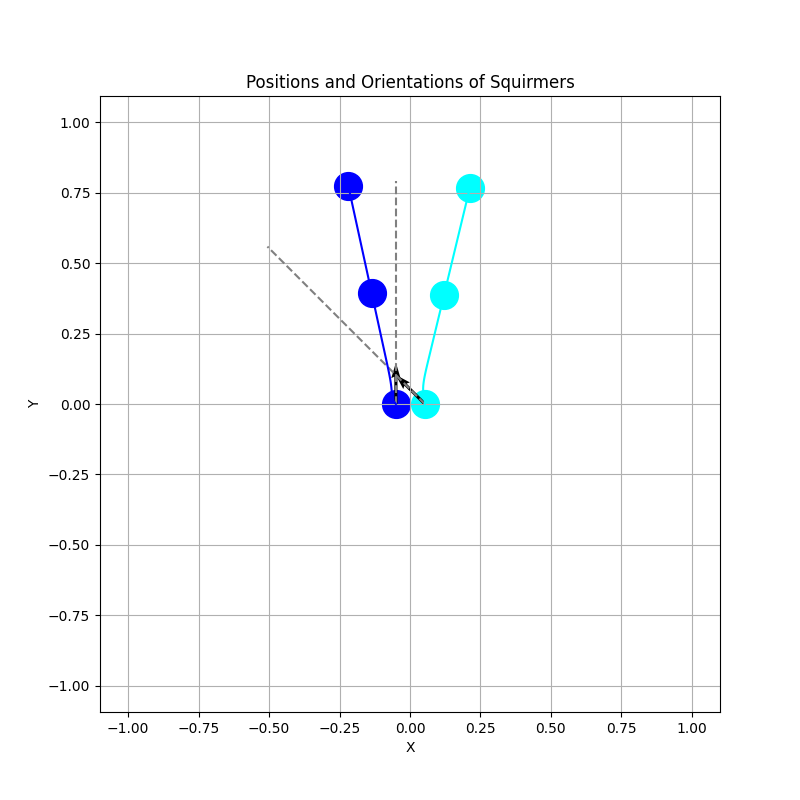
\includegraphics[width=1\textwidth]{../../graphs/simulations/sim_sq_sq/betam3/3pi_4_.png}
        $\beta = -3$
    \end{minipage}
\end{frame}

\begin{frame}{Numerical Experiments}
    \framesubtitle{Simulation of two interacting squirmers}
    \begin{center}
        \textbf{$\theta_2 = \pi$}
    \end{center}
    \begin{minipage}{0.49\textwidth}
        \centering
        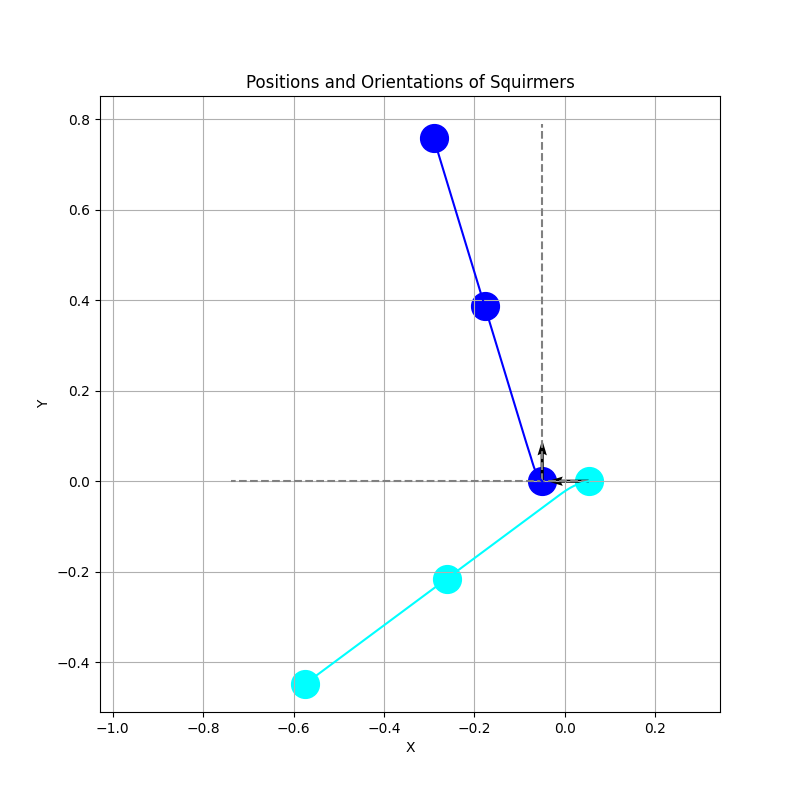
\includegraphics[width=1\textwidth]{../../graphs/simulations/sim_sq_sq/betam1_5/pi_.png}
        $\beta = -1.5$
    \end{minipage}
    \begin{minipage}{0.49\textwidth}
        \centering
        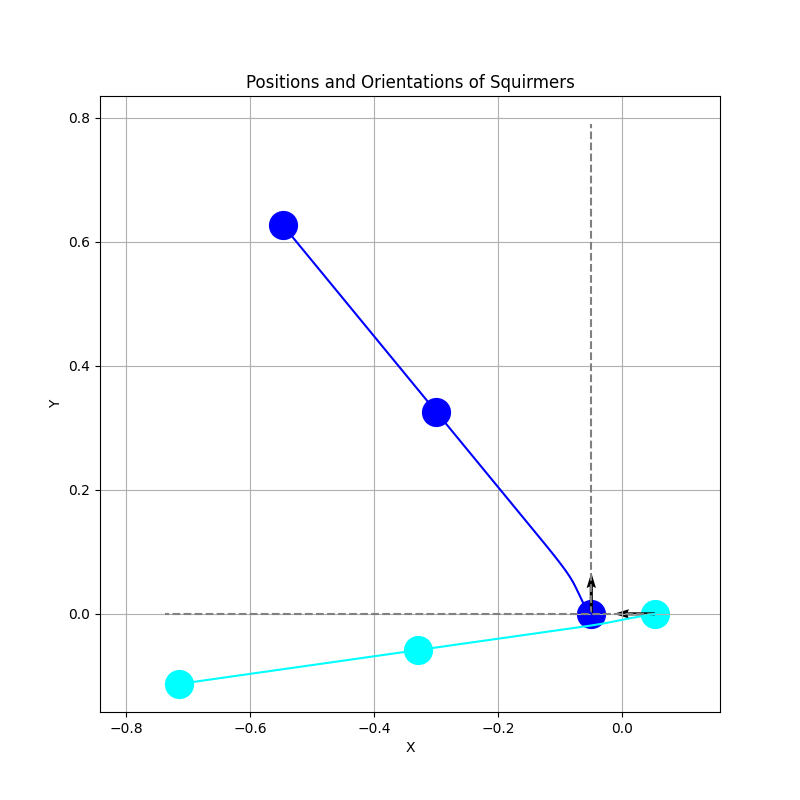
\includegraphics[width=1\textwidth]{../../graphs/simulations/sim_sq_sq/beta1_5/pi_.png}
        $\beta = 1.5$
    \end{minipage}
\end{frame}

\begin{frame}{Numerical Experiments}
    \framesubtitle{Simulation of two interacting squirmers}
    \centering
    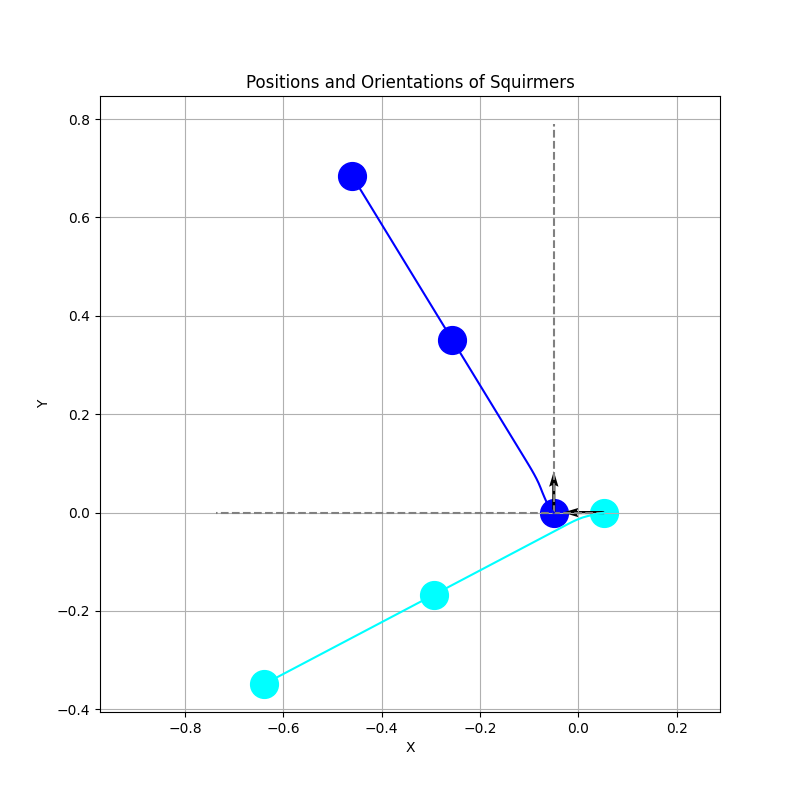
\includegraphics[width=0.5\textwidth]{../../graphs/simulations/sim_sq_sq/beta0/pi_.png}
    \begin{center}
        $\beta = 0$
    \end{center}
\end{frame}

\begin{frame}{Numerical Experiments}
    \framesubtitle{Simulation of squirmer-border interaction}
    \begin{center}
        \textbf{$\theta = -\frac{\pi}{4}$}
    \end{center}
    \begin{minipage}{0.49\textwidth}
        \centering
        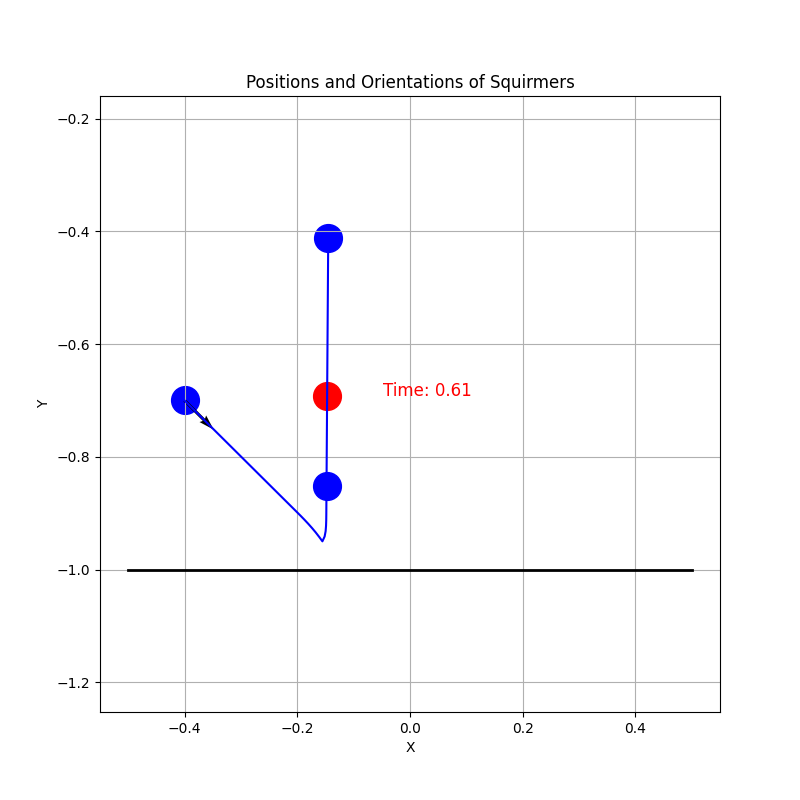
\includegraphics[width=1\textwidth]{../../graphs/simulations/border/betam1_5/mpi_4.png}
        $\beta = -1.5$
    \end{minipage}
    \begin{minipage}{0.49\textwidth}
        \centering
        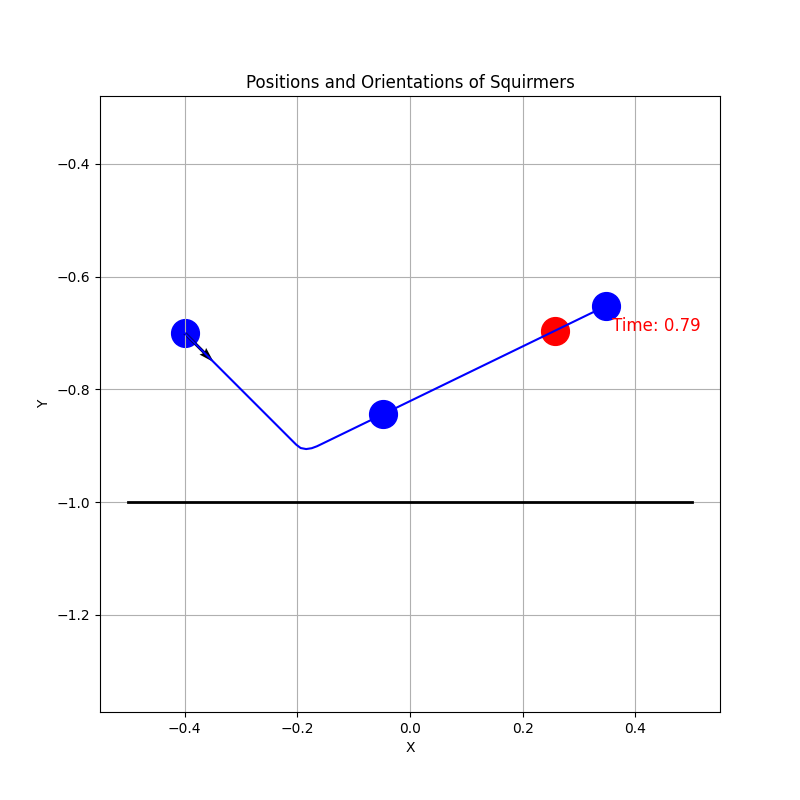
\includegraphics[width=1\textwidth]{../../graphs/simulations/border/beta1_5/mpi_4.png}
        $\beta = 1.5$
    \end{minipage}
\end{frame}

\begin{frame}{Numerical Experiments}
    \framesubtitle{Simulation of squirmer-border interaction}
    \centering
    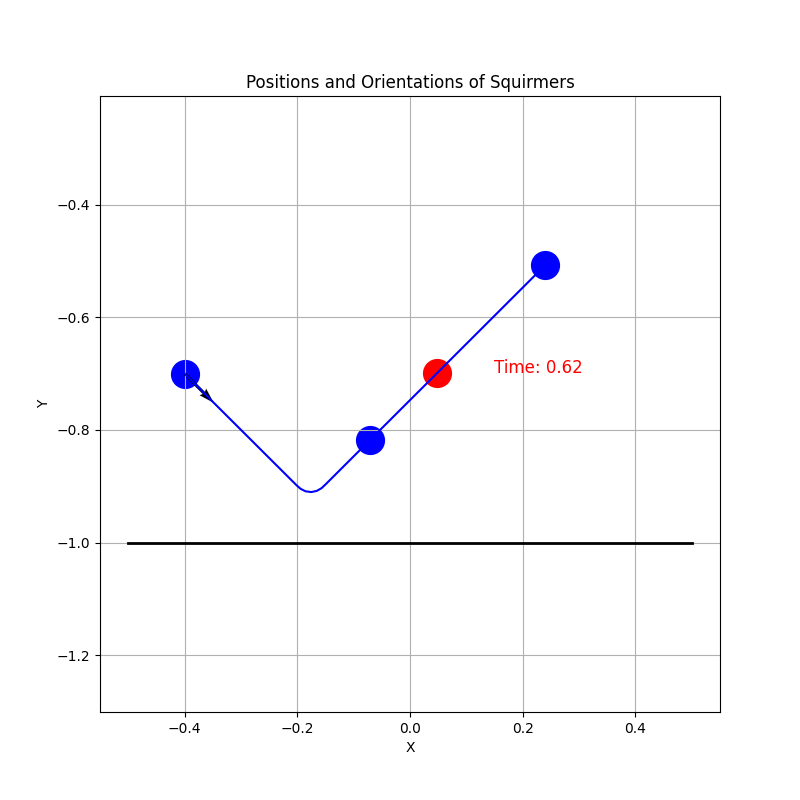
\includegraphics[width=0.5\textwidth]{../../graphs/simulations/border/beta0/mpi_4.png}
    \begin{center}
        $\beta = 0$
    \end{center}
\end{frame}

\begin{frame}{Numerical Experiments}
    \framesubtitle{Simulation of squirmer-border interaction}
    \begin{center}
        Two different positive $\beta$ values
    \end{center}
    \begin{minipage}{0.49\textwidth}
        \centering
        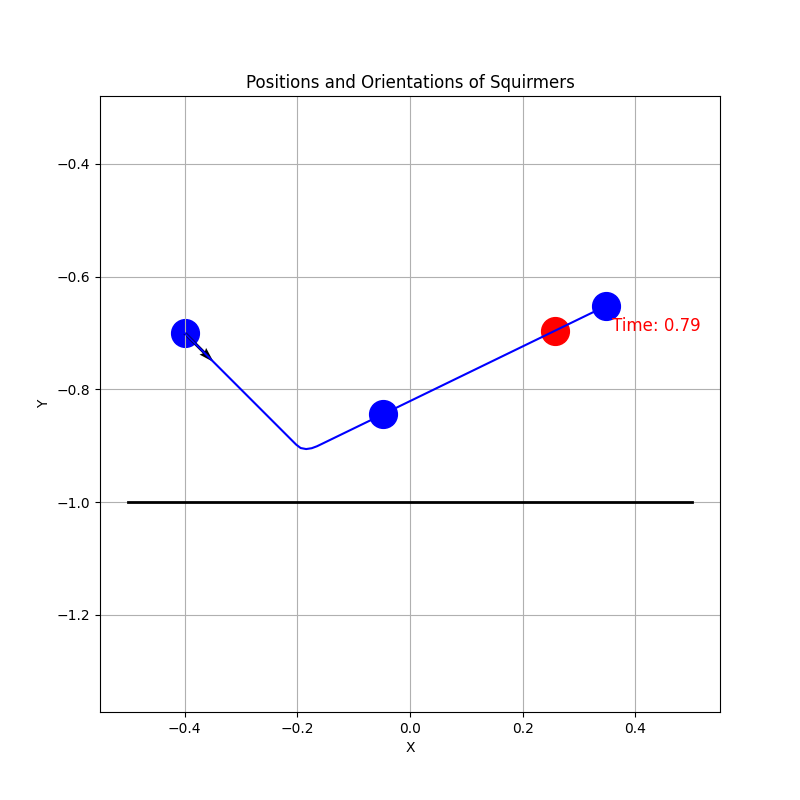
\includegraphics[width=1\textwidth]{../../graphs/simulations/border/beta1_5/mpi_4.png}
        $\beta = 1.5$
    \end{minipage}
    \begin{minipage}{0.49\textwidth}
        \centering
        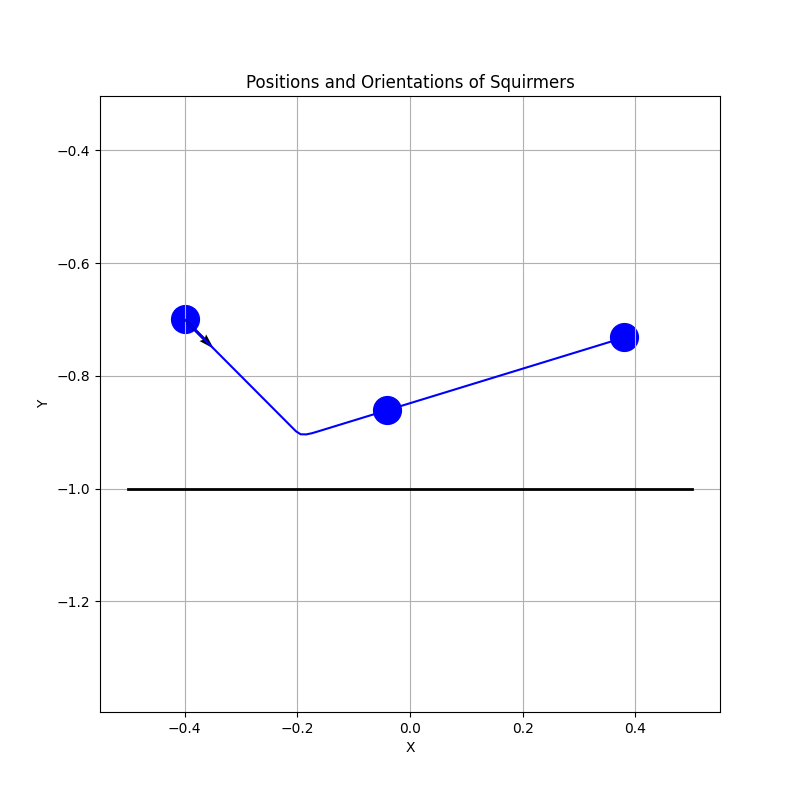
\includegraphics[width=1\textwidth]{../../graphs/simulations/border/beta3/mpi_4.png}
        $\beta = 3$
    \end{minipage}
\end{frame}

\begin{frame}{Numerical Experiments}
    \framesubtitle{Simulation of squirmer-border interaction}
    \begin{center}
        Two different negative $\beta$ values
    \end{center}
    \begin{minipage}{0.49\textwidth}
        \centering
        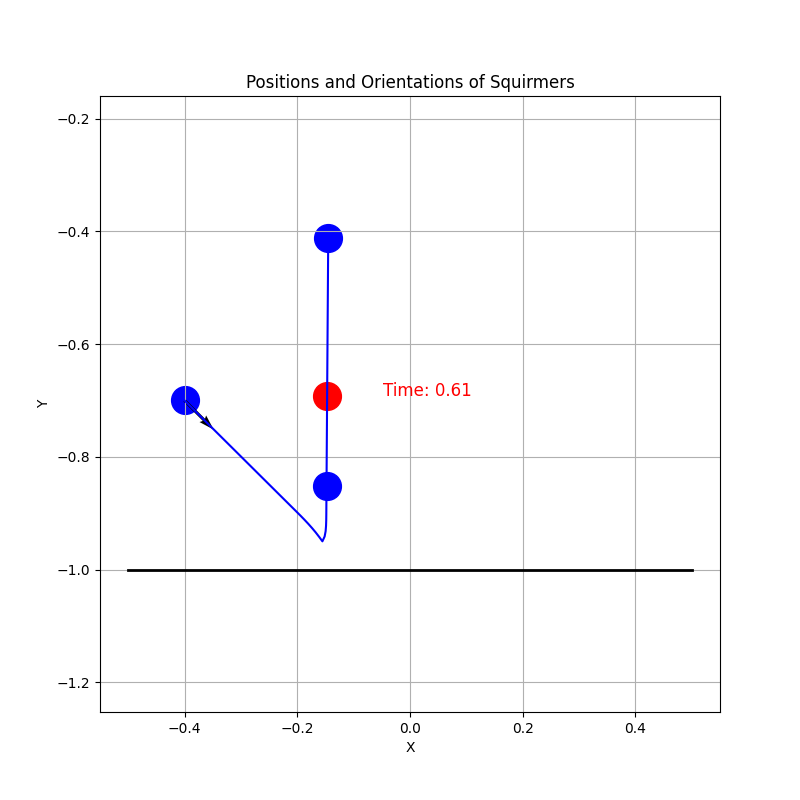
\includegraphics[width=1\textwidth]{../../graphs/simulations/border/betam1_5/mpi_4.png}
        $\beta = -1.5$
    \end{minipage}
    \begin{minipage}{0.49\textwidth}
        \centering
        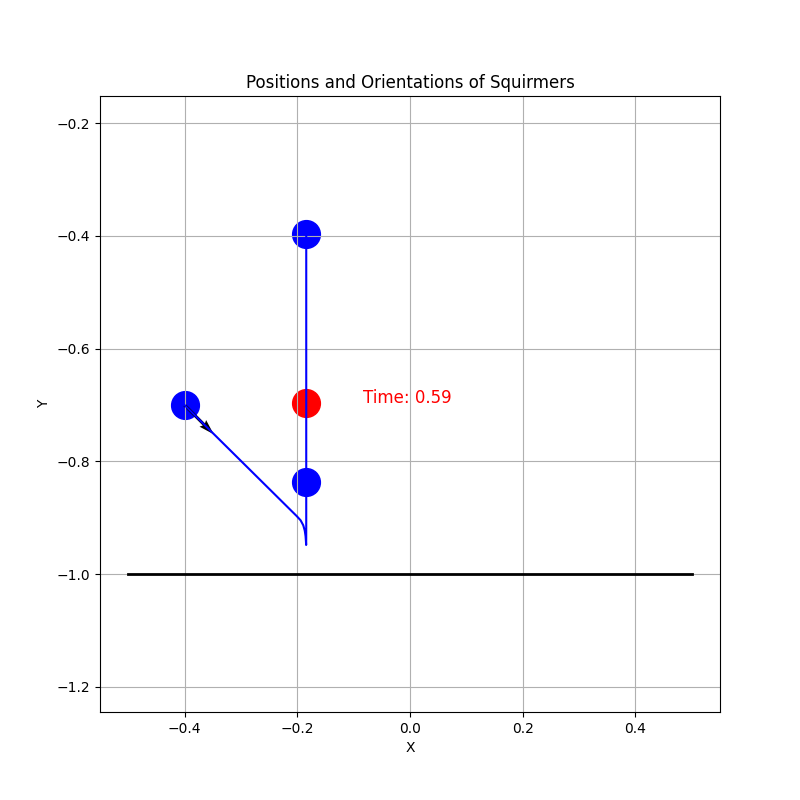
\includegraphics[width=1\textwidth]{../../graphs/simulations/border/betam3/mpi_4.png}
        $\beta = -3$
    \end{minipage}
\end{frame}

\section{N squirmers}
\begin{frame}{N squirmers}
    \href{https://youtu.be/Uy90m-Cd2AA}{Video of 375 squirmers in a box}\\
    \href{https://www.youtube.com/watch?v=wKGb-HLe0Ik}{Video of 375 squirmers in a channel}
\end{frame}

\section{Simulation of 375 squirmers by varying the D parameter}
\begin{frame}{Simulation of 375 squirmers by varying the D parameter}
    
\end{frame}

\section{Conclusion and perspective}
\begin{frame}{Conclusion and perspective}
    \begin{center}
        \begin{itemize}
            \item Varying $\beta$ value affect behavior
            \item Convergence of results with $\beta = 0$
            \item Discrepancy of results for $\beta \ne 0$
            \item Investigating the interactions within a shoal of squirmers : collective behavior and emergent group effects
        \end{itemize}
    \end{center}
\end{frame}

\section{References}
\begin{frame}{References}
    \begin{thebibliography}{}
        \bibitem{Brumley} D.R. Brumley and T.J. Pedley, \emph{Stability of arrays of bottom-heavy spherical squirmers}, American Physical Society, 2019
        \bibitem{Lauga} Théry A., Maaß C.C. and Lauga E., \emph{Hydrodynamic interactions between squirmers near walls: far-field dynamics and near-field cluster stability}, Royal Society Open Science, 2023
        \bibitem{Stark} Miloš Knežević,Till Welker \& Holger Stark, \emph{Collective motion of active particles exhibiting non-reciprocal orientational interactions}, Scientific Reports, 2022
        \bibitem{Wikipedia} Wikipédia, \emph{Squirmer}, Wikipédia, 2022
    \end{thebibliography}
\end{frame}

\end{document}